% !TEX TS-program = pdflatex
% !TEX encoding = UTF-8 Unicode

% This is a simple template for a LaTeX document using the "article" class.
% See "book", "report", "letter" for other types of document.

\documentclass[11pt,twocolumn]{article} % use larger type; default would be 10pt

\usepackage[utf8]{inputenc} % set input encoding (not needed with XeLaTeX)

%%% Examples of Article customizations
% These packages are optional, depending whether you want the features they provide.
% See the LaTeX Companion or other references for full information.

%%% PAGE DIMENSIONS
\usepackage{geometry} % to change the page dimensions
\geometry{a4paper, margin=0.5in} % or letterpaper (US) or a5paper or....
% \geometry{margin=2in} % for example, change the margins to 2 inches all round
% \geometry{landscape} % set up the page for landscape
%   read geometry.pdf for detailed page layout information

\usepackage{graphicx} % support the \includegraphics command and options
\usepackage{mathtools}
\usepackage{amsmath} % need this stuff for curly brackets
% \usepackage[parfill]{parskip} % Activate to begin paragraphs with an empty line rather than an indent

%%% PACKAGES
% Nice package for plotting graphs
% See excellent guide:
% http://www.tug.org/TUGboat/tb31-1/tb97wright-pgfplots.pdf
\usepackage{pgfplots}
\usetikzlibrary{plotmarks}

\usepackage{pgfplots} % Plots
\usepackage{pgfplotstable} % Tables
\usepackage{xcolor} % To color text
\usepackage[official]{eurosym} % Euro symbol
\usepackage{booktabs} % for much better looking tables
\usepackage{array} % for better arrays (eg matrices) in maths
\usepackage{paralist} % very flexible & customisable lists (eg. enumerate/itemize, etc.)
\usepackage{verbatim} % adds environment for commenting out blocks of text & for better verbatim
\usepackage{subfig} % make it possible to include more than one captioned figure/table in a single float
\usepackage{authblk}
\usepackage{pdfpages}
\usepackage{wrapfig}
\usepackage{hyperref}
\hypersetup{
    colorlinks,
    citecolor=black,
    filecolor=black,
    linkcolor=black,
    urlcolor=black
}
\usepackage{listings}
\lstset{frame=tb,
  language=BASH,
  aboveskip=3mm,
  belowskip=3mm,
  showstringspaces=false,
  columns=flexible,
  basicstyle={\small\ttfamily},
  numbers=none,
  numberstyle=\tiny\color{gray},
  keywordstyle=\color{blue},
  commentstyle=\color{dkgreen},
  stringstyle=\color{mauve},
  breaklines=true,
  breakatwhitespace=true
  tabsize=1
}
% These packages are all incorporated in the memoir class to one degree or another...

%%% HEADERS & FOOTERS
\usepackage{fancyhdr} % This should be set AFTER setting up the page geometry
\pagestyle{fancy} % options: empty , plain , fancy
\renewcommand{\headrulewidth}{0pt} % customise the layout...
\lhead{}\chead{}\rhead{}
\lfoot{}\cfoot{\thepage}\rfoot{}

%%% SECTION TITLE APPEARANCE
\usepackage{sectsty}
\allsectionsfont{\sffamily\mdseries\upshape} % (See the fntguide.pdf for font help)
% (This matches ConTeXt defaults)

%%% ToC (table of contents) APPEARANCE
\usepackage[nottoc,notlof,notlot]{tocbibind} % Put the bibliography in the ToC
\usepackage[titles,subfigure]{tocloft} % Alter the style of the Table of Contents
\renewcommand{\cftsecfont}{\rmfamily\mdseries\upshape}
\renewcommand{\cftsecpagefont}{\rmfamily\mdseries\upshape} % No bold!

%%% END Article customizations

\title{Parallel Algorithms \\ Classified Assignment}
\author{Wael Aljeshi\thanks{wael.aljeshi10@imperial.ac.uk}}
\author{Dan Demeter\thanks{dan.demeter10@imperial.ac.uk}}
\author{Razvan Rosie\thanks{razvan.rosie10@imperial.ac.uk}}
\affil{Department of Computing, Imperial College London}

\begin{document}
\maketitle

\renewcommand{\abstractname}{Mission Brief}

\begin{abstract}
A top secret computer system was discovered by extraction squad 429 in the nation of Nukehavistan. Highly detailed snapshots of the machine in operation were handed over, as well as a software implementation of the retrieved circuit board, residing in \texttt{mystery.o}. This report, addressed to the Director of Secret Services\footnote{Sir Robert Hinchcliffe-Smythers-Smythe the 3rd}, details the methodologies of our mission and our findings.
\end{abstract}



\section{Investigating the machine}
The forensics team started by investigating the physical exterior of the machine, looking for clues which may allude to its function. This section discusses their methodologies and findings in detail.


\subsection{Technical number enquires}

\begin{figure}[h]
	\centering
	
\includegraphics[width=0.8\columnwidth]{img/phone-enquiries.jpg}
	\caption{Technical enquiries phone number}
	\label{fig:technical-enquiries}
\end{figure}

The message in Figure~\ref{fig:technical-enquiries} was prominently displayed near the top of the machine. A look up of historical phone directory records traced the number back to the \emph{ORSA Journal on Computing}. 
A follow up visit was made to their customer services branch (Figure~\ref{fig:orsa-map}):

\begin{quote}
5521 Research Park Drive \\
Suite 200 \\
Catonsville, Maryland 21228-4664 \\
USA
\end{quote}

\begin{figure}[h]
	\centering
	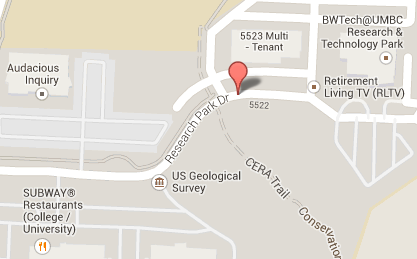
\includegraphics[width=0.95\columnwidth]{img/orsa.png}
	\caption{ORSA Journal on Computing customer services branch. Brunch was purchased from \protect 
\includegraphics[height=0.98em,keepaspectratio]{img/subway.png}.}
	\label{fig:orsa-map}
\end{figure}

The team was then able to retrieve an excerpt\footnote{An online version was independently found at \url{http://www.columbia.edu/~ww2040/Fall03/LaplaceInversionJoC95.pdf}} of a document \emph{Numerical Inversion of Laplace Transforms of Probability Distributions}.


\subsection{Cyrillic script}
Some Cyrillic script was found on the machine, believed by our Business and Strategy experts to be used for marketing the machine in the Russian market.

An image of the script was analysed and translated electronically (Figure~\ref{fig:cyrillic-script}), yielding the rough English translation of \emph{Fast inverter integrated functions}.

\begin{figure}[h]
	\centering
	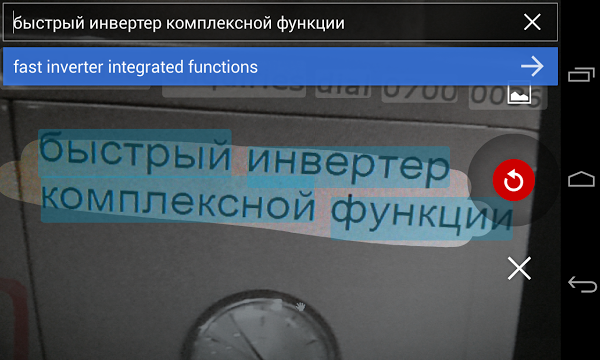
\includegraphics[width=0.9\columnwidth]{img/cyrillic-script.png}
	\caption{Cyrillic script found on the machine, along with the analysis results.}
	\label{fig:cyrillic-script}
\end{figure}

It is speculated that this marketing campaign was highly unsuccessful, as the marketing text consisted merely of a catchy phrase with no detailed description of operation \footnote{Catchy marketing phrases are clearly an inferior marketing technique, and would never work --- c.f. ``Just do it'' and ``I'm lovin' it'' for examples of such unsuccessful campaigns.}. Additionally, the provided help instructions were provided in a crude mixture of English and French, probably unhelpful for the Russian operators.




\subsection{Geographic coordinates}
The geographic coordinates $2.3328700E \; 48.8074800N$ were found inscribed on the machine. However, due to a lack of 3G signal in the basement, the geographic team were unable to access the internet and hence encountered difficulties in determining the whereabouts of the coordinates inscribed on the machine. The issue was promptly escalated to the CTO, who commissioned the purchase of two horses from a local supermarket. \footnote{Despite the falling price of petrol, it remains beyond our budget. As a plus, horses are also free to park.}

The location was found to be near the Laplace train station in France (Figure~\ref{fig:laplace-horses}). Realising the mismatch in units due to the ``inverse function'' applied to the coordinates, the agents determined that the devious scheme was intended to be a very subtle hint that the machine may be performing an inverse Laplace transform. In order to cut costs, the horses were auctioned off at the nearby \emph{Square du Serment de Koufra} for a profit of \EUR{7.89}. This was sufficient to purchase baguettes for lunch.

\begin{figure}[h]
	\centering
	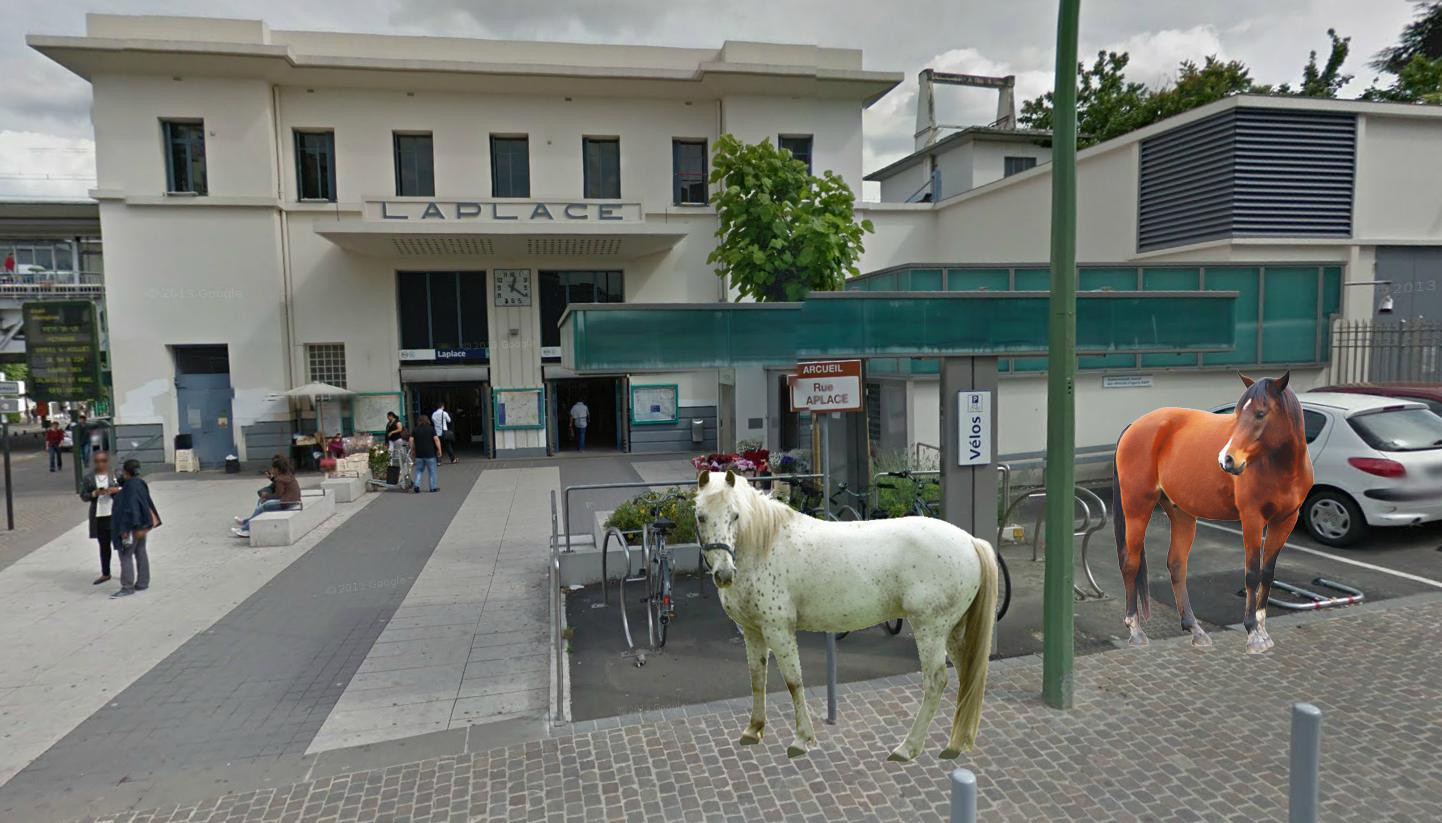
\includegraphics[width=0.95\columnwidth]{img/laplace-horses.jpg}
	\caption{Straight ahead: the main entrance of the Laplace train station. Right: the parked horses.}
	\label{fig:laplace-horses}
\end{figure}



\subsection{Portrait}
% Google colors
\definecolor{google-blue}{HTML}{0266C8}
\definecolor{google-red}{HTML}{F90101}
\definecolor{google-yellow}{HTML}{F2B50F}
\definecolor{google-green}{HTML}{00933B}
\newcommand{\google}{\textcolor{google-blue}{G}\textcolor{google-red}{o}\textcolor{google-yellow}{o}\textcolor{google-blue}{g}\textcolor{google-green}{l}\textcolor{google-red}{e}}

A grayscale portrait was located on the central axis of the machine (Figure~\ref{fig:euler}). As the portrait's CMYK band was much too narrow for our forensic experts' eyes, an image was instead captured and sent to the \textcolor{google-blue}{G}l\textcolor{google-red}{O}bal cl\textcolor{google-yellow}{O}ud-based \textcolor{google-blue}{G}enealogy \textcolor{google-green}{L}ocator \textcolor{google-red}{E}-service (\google). The subject was identified as Leonhard Euler,``a pioneering Swiss mathematician and physicist'' (according to an omni-reliable, omni-malleable source \footnote{Wikipedia, the free encyclopedia}). This may hint that the machine employs Euler's methods for its computation.

\begin{figure}[h]
	\centering
	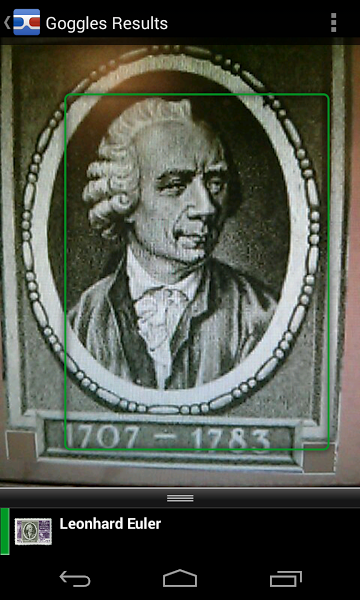
\includegraphics[width=0.8\columnwidth]{img/euler.png}
	\caption{The result of the analysis on the portrait reveals the subject to be Leonhard Euler.}
	\label{fig:euler}
\end{figure}



\subsection{Wall clock and CRT Display}

The machine panel has two seemingly, and deceivingly, unrelated components.

\begin{figure}[h]
	\centering
	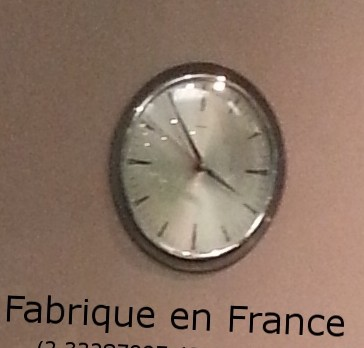
\includegraphics[width=0.8\columnwidth]{img/clock.jpg}
	\caption{The wall clock located on the main panel of the machine}
	\label{fig:clock}
\end{figure}

Firstly we have the wall clock (Figure ~\ref{fig:clock}), indicating the current time (as clocks do) to be $3:55$, or more likely $15:55$ given the sunlight in the background. Since Nukehavistan is located around $31N$ latitude (Figure~\ref{fig:map}), we are not dealing with a case of midnight sun\footnote{\url{http://en.wikipedia.org/wiki/Midnight_sun}}.

\begin{figure}
	\centering
	
\includegraphics[width=0.8\columnwidth]{img/nukehavistan.jpg}
	\caption[A map of the Republic of Nukehavistan]{A map of the Republic of Nukehavistan \protect \footnotemark}
	\label{fig:map}
\end{figure}
\footnotetext{Image courtesy of The Onion \\ \url{http://www.theonion.com/articles/us-intelligence-nukehavistan-may-have-nuclear-weap,1373/}}


Secondly we have the CRT display (Figure~\ref{fig:crt}), which shows a graph of some function $f(t)$ over time. The graph has a positive peaks at $t = 3$ and a negative peak at $t = 11$. 

\begin{figure}[h]
	\centering
	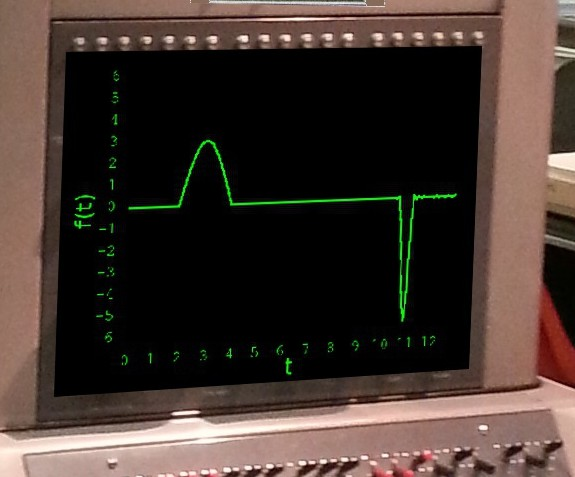
\includegraphics[width=0.8\columnwidth]{img/crt.jpg}
	\caption{The CRT display showing a live graph in neon-ish green.}
	\label{fig:crt}
\end{figure}

After copious degrees of analysis, it was determined that the peaks in the graph are actually mirroring the hands of the clock, the positive peak representing the position of the hour hand (rounded down to the current hour), and the negative peak representing the position of the minute hand (rounded down to the nearest multiple of five). The fact that the $t$ axis runs from $0$ to $12$ further supports this argument. Thus the graph in the image points at $3$ (as is the current hour) and $11$, translating to minutes $55-59$ (as is the current minute).

The circuit board is therefore used to plot a curve representing the current (12-hour) time (Figure~\ref{fig:essentially}).

\begin{figure}[h]
	\centering
	
\includegraphics[width=0.8\columnwidth]{img/essentially.jpg}
	\caption{Fox news anchor Megyn Kelly commenting on the discovery.}
	\label{fig:essentially}
\end{figure}

Our agent from the "Hidden special unit for reverse analysis and decompilation" was able to successfully decompile the mysterious `mistery.o` file and write the equivalent C++ code. Further testing combined with the latest research in the filed of Reasoning about programs confirmed that our code produces exactly the same results as the initial object file. Below are the pseudo-code function calls that are used to compute the final answer: 

-- insert here the pseudo-code for functions ---

We would like to report some anomalies we have detected in the file, which we believe that have been put in place by the circuit designer in order to make the disassembly process more difficult:

\begin{itemize}
 \item Extra strings.
 We have noticed 2 ambiguous strings written at the beginning of the file: <INSERT HERE THE STRINGS>. They provide some insights into who wrote the initial software and the year it might have been written. 
 \item $y = (x)^782768$, where x = 0.99999999999999 
 Due to the fact that 0.99999999999999 < 1 and because floating point numbers can't be represented exactly by the 64bit processors, the results of this multiplication will be 0. Throughout the run of our program we have determined that the x values never changes so the result is always 0.
 \item stdlib sincos(x) and log(x + 1) functions
 The argument for the sincos function is y and (y + 1) for the log function, where y is the results of the multiplication discussed above. Because y is constant, sincos(y) returns (0,1) and log(y+1) returns 0;
 \item Bogus while loops
 During the research our agent has identified 4 repetitive structures. One repetitive structure is used to compute $y = (x)^782768$ in a very ineffective way. The other 2 repetitive structures have the same implementation and they serve as iterators through the 2 initial strings defined in the program. Their main purpose is to compute the offset between a specific ASCII character ( 0x80 ) and the initial strings. Because the strings are hard-coded, the results computed by both the strings will be always 35 ( 0x23 ) and 49 ( 0x31 ). 
 Lastly, the 4th structure is the "main" while loop. The repetitive condition for this loop is as follows: $(0x31 + sin(y) + cos(y) + log(1+y) - 29 - 48 + y) > 20$, which simplifies to $(7 + sin(y) + cos(y) + log(1+y) > 20)$. Because y is a constant (0), $log(1+y) + sin(y) + cos(y)$ will be 1, so the loop condition is will never be true $8 > 20$.
 Our agent is not sure whether these assembly artifacts and a lot of hard-coded values have been inserted in order to trick us or the compiler just generated general purpose code. 
 \item Compiler uses the stack base pointer (RBP)
 During the analysis, it has been found that the L() function does not properly set the stack base pointer and instead it uses it as a general purpose register. This implies the fact that new variables are not created on the stack. The compiler is aware at compile time of the total number of variables used in the program and this is a known technique used by compilers in such situations. 
  
\end{itemize}

During the decompilation process our agent has used a test-driven approach, by writing scripts that would automate testing our computed function against the original "mistery.o" one. We used the program \textbf{faketime} in order to generate 1440 tests cases: 1 test for each minute in a day. Then we used a parallel diff program that would call both our function and the original L() one with different parameters and report any different results. Part of the tools used by the agent were the GNU Debugger gbd, with the peda plugin and the IDA program. No automated tools have been used ( because there is none for 64bit programs ).

\section{Investigating the circuit}
The next step was to investigate the pluggable circuit board, the process and results of which are discussed in this section.

\subsection{Circuit board macro-analysis}
The circuit board itself was identified as a product of AMD, housing a 500 MHz AMD Geode LX800 and 256 MB DDR DRAM (Figure~\ref{fig:circuit-board}). Such technology was not believed to exist at the time, and it seems that great efforts have been devoted to keep this technology hidden.


\begin{figure}[h]
    \centering
    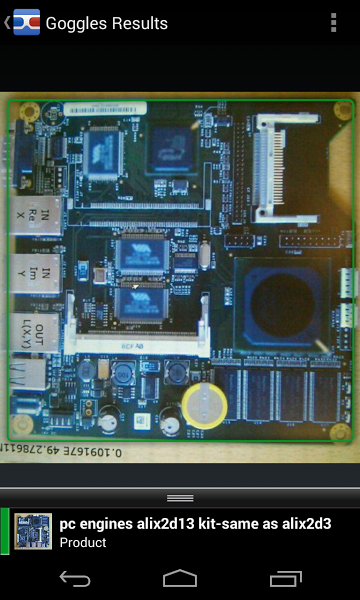
\includegraphics[width=0.8\columnwidth]{img/circuit-board.png}
    \caption{The identified circuit board}
    \label{fig:circuit-board}
\end{figure}

This leaves investigating yet another set of geographic coordinates: $0.109167E \; 49.278611N$. Learning from their previous experience, the geographic team decided to book a flight this time. They, of course, did not learn from their \emph{other} mistake, and hence spent quite some time travelling instead of taking the more sensible option of employing a parallel depth first search on the earth's map. The fact was reflected appropriately in their performance review. But we digress \ldots

\begin{figure}[h]
    \centering
    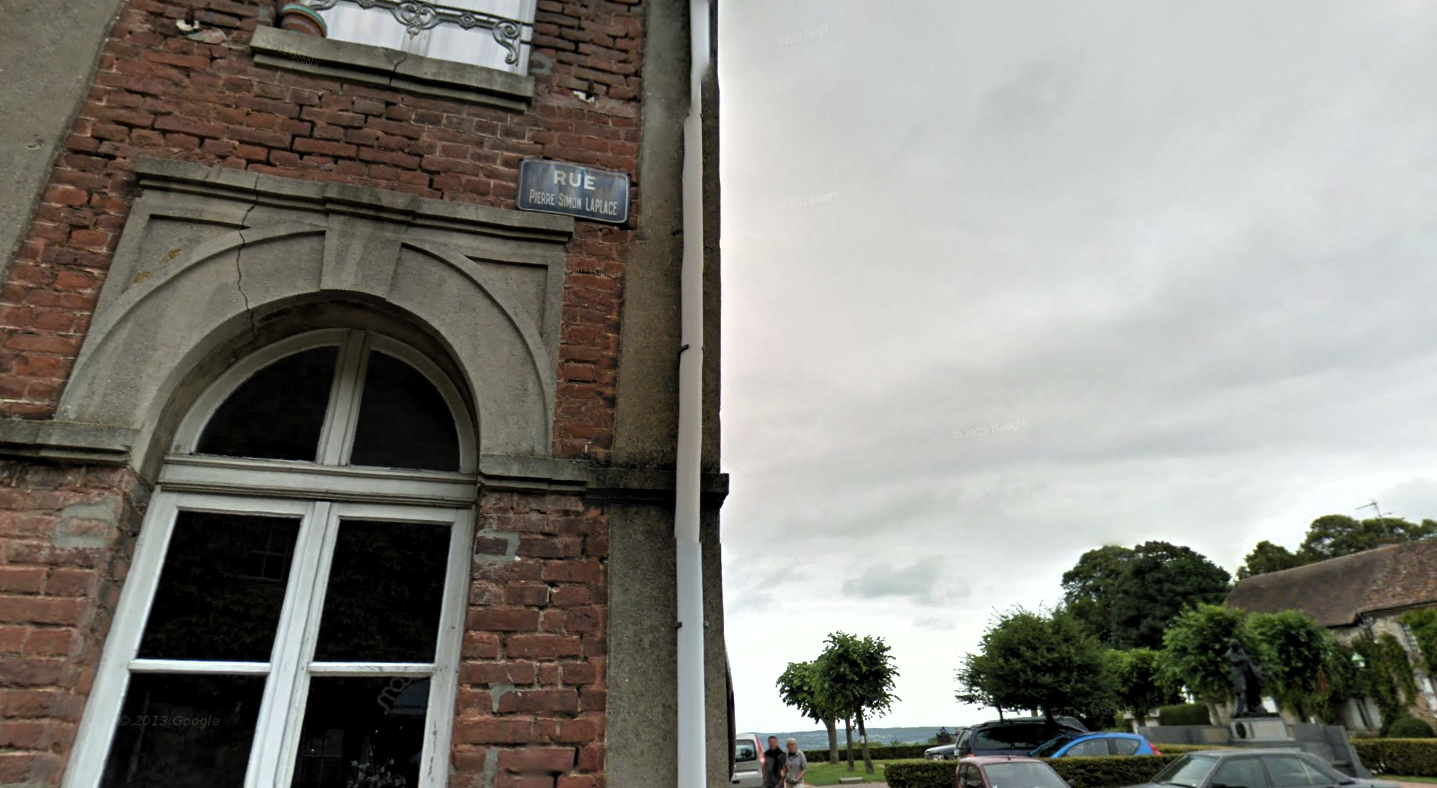
\includegraphics[width=0.95\columnwidth]{img/laplace-road.png}
    \caption{Rue Pierre Simon Laplace Road - You will never find a more blessed hive of charm and harmony}
    \label{fig:laplace-road}
\end{figure}


After an expensive trip to France, it was determined that the site referred to ``Ecole Beaumont en auge'' at ``Rue Pierre Simon Laplace Road'' (Figure~\ref{fig:laplace-road}). The connection was made the following week, when the team realised that the circuit was meant to employ some form of Laplace transform.


\subsection{Circuit board microanalysis}

With the macro analysis out of the way, our experts studied the circuit board's functionality through means of the reconstructed \texttt{mystery.o} object file.



\subsubsection{\texttt{strings} analysis}
Executing \texttt{strings} analysis on \texttt{mystery.o} revealed the following hidden data:

\begin{quote}
\texttt{(C) 2006 Svenska Aeroplan AB (SAAB) Designad av Margarita Gonz\'{a}lez Sampayo, Linkoping}
\end{quote}

The English translation:
\begin{quote}
\texttt{(C) 2006 Swedish Aeroplane Company Limited (SAAB) Designed by Margarita Gonz\'{a}lez Sampayo, Linkoping}
\end{quote}


A background search revealed that Dr. Margarita Holmberg (Gonz\'{a}lez Sampayo was her maiden name) had centred her PhD thesis\footnote{Engineering problem solving
- The case of the Laplace transform as a difficulty in learning in electric circuits and as a tool to solve real world problems} around the Laplace Transform in electric circuits. Indeed, it seems that SAAB is mentioned twice in her thesis, in the context of a practical application of the Laplace transform:

\begin{quote}
To solve problems working in Companies applying automatic control (for example, working in SAAB with aircraft dynamics) you use the Laplace transform.
\end{quote}




\subsubsection{\texttt{objdump} analysis}
The symbol table of \texttt{mystery.o} was extracted using \texttt{objdump --syms}. This revealed a number of interesting library functions being used:
\begin{itemize}
\item Mathematical functions, often operating on complex numbers, such as \texttt{cexp}, \texttt{muldc3}, \texttt{log}, and others.
\item Time-related functions, \texttt{time}, \texttt{strftime}, \texttt{strtol}, and \texttt{localtime})
\end{itemize}

Whilst the mathematical functions were to be expected, the time-related functions came as a surprise to our agents. This discovery motivated further, more dynamic, investigation.


\subsubsection{\texttt{ltrace} analysis}
By running \texttt{ltrace} whilst running the team obtained the library calls used during the computation phase. The first and subsequent runs are almost identical, apart from an extra initialisation step. The initialisation step includes a call to \texttt{localtime}, protected by \texttt{cxa\_guard} calls, which are used ``to support thread-safe, one-time initialisation of function scope variables''\footnote{\url{http://www.opensource.apple.com/source/libcppabi/libcppabi-14/src/cxa_guard.cxx}} (Figure~\ref{fig:l-calls}).


\begin{figure}[h]
    \centering

    \begin{tabular}{cc}
    \toprule
    Initial call & Subsequent calls \\

    \midrule

    \texttt
        time                                    & time        \\
        {\color{red} \_\_cxa\_guard\_acquire }  &             \\
        {\color{red} localtime }                &             \\
        {\color{red} \_\_cxa\_guard\_release }  &             \\
        strftime                                & strftime    \\
        strftime                                & strftime    \\
        strtol                                  & strtol      \\
        strtol                                  & strtol      \\
        \_\_muldc3                              & \_\_muldc3  \\
        cexp                                    & cexp        \\
        cexp                                    & cexp        \\
        \_\_divdc3                              & \_\_divdc3  \\
        \_\_muldc3                              & \_\_muldc3  \\
        \_\_muldc3                              & \_\_muldc3  \\
        sincos                                  & sincos      \\
        log                                     & log         \\
        cexp                                    & cexp        \\
        \_\_divdc3                              & \_\_divdc3  \\
        \_\_muldc3                              & \_\_muldc3  \\
        cexp                                    & cexp        \\
        \_\_muldc3                              & \_\_muldc3  \\
    \bottomrule
    \end{tabular}

    \caption{Trace of library calls for the initial and subsequent calls of the function \texttt{L()} . The extra library calls performed in the first function call are highlighted in red.}
    \label{fig:l-calls}
\end{figure}


\section{Serial Implemantation}
After agreeing that the machine is in fact an inverter of $Laplace$ transforms, some time was spent investigating 
this mathematical concept. Directly, the transform can be given in the following way:
$$F(s) =\int_0^\infty \! f(t)e^{-st} \, \mathrm{d}t$$

Since we have established that we need to find the inverse transform, we notice the fact that:
$$f(t) =\int_0^\infty \! F(s)e^{st} \, \mathrm{d}t$$
\newline

To recap the data which we have gathered so far, the agents are facing the following problems:
\begin{itemize}
\item{The analytical expression of the function $F$ given by $mystery.o$ is unknown. }
\item{The $mistery.o$ file only allows for evaluation of the function at some points passed as inputs. }
\end{itemize}

Therefore, we have realised that we need to perform numerical inverse of $Inverse$ $Laplace$ $transform$.
The paper offered us a valuable introduction to the problem that we were facing.
The \texttt{EULER} algorithm was a starting point, and we proceed to the implementation step:

\subsection{EULER Algorithm}
The best description\cite{abate} of the \texttt{EULER} algorithm can be summarised by the formula:
$$f(t) = \frac{10^{M/3}}{t} \sum\limits_{k=0}^{2M} {\eta_k Re F(\frac{\beta_k}{t}) }$$
Where:
$$\beta_k = \frac{M ln(10)}{3} + i\pi k$$
$$\eta_k = (-1)^{k} *\xi_k$$
$$\xi_0 = \frac{1}{2}$$
$$\xi_k = 1 \text{for} 1 \leq k \leq M$$
$$\xi_{2M} = \frac{1}{2M}$$
$$\xi_{2M-k} = \xi_{2M-k+1}+2^{-M}\binom{M}{k}$$
\newline

The implementation of the algorithm follows the procedure described above and can be described the following manner:
\begin{itemize}
\item{Select a size for the parameter M (for the current problem we use M as 30).}
\item{Define an array \texttt{Times} to store the arguments where of the targeted function $f$.}
\item{Construct an array of factors ($\xi$) which will act as factors in the summation of $F(\frac{\beta_k}{t})$. Set $xi[0] = 1/2$. Fill the elements on positions $1$ $\to$ $M+1$ with 1s. Fill the rest of the array with the factors of the binomial expansion of order $2M$, as presented above.}
\item{Precompute the constants described by the algorithm.}
\item{For each point of time $t$, compute the sum described by the algorithm. This part of the code operates in an independent way (since we compute the sum for each point) and is suitable for a parallel implementation.}
\item{Output the vector $f_{st}$ containing the results of the evaluations.}
\end{itemize} 

Our serial implementation described the same graph as the one shown, with its global maxima pointing the hour and the global minima pointing the minute.


\subsection{The Dubner-Abate Algorithm}
After making sure that the \texttt{EULER} method works, the team decided to test other algorithms in order to compare the results and efficiency.
We present here the $Dubner \& Abate$ algorithm, which is also computes the inverse of a $Laplace$ transform as a $Fourier$ cosine series.
The mathematics behind this algorithm are simpler because it does not require the computation of the binomial coefficients (which involve factorials) and may produce overflows.

In short, the $Dubner$-$Abate$ algorithm will compute the following:
\begin{align*}
f(t) = \frac{e^{At}}{q} \sum\limits_{k=1}^{M}{Re(L(A+t\frac{ki\pi}{q}) \cdot cos(t\frac{k\pi}{q}))} \\
- \sum\limits_{k=1}^{M}{Im(L(A+t\frac{ki\pi}{q}) \cdot sin(t\frac{k\pi}{q}) )}
\end{align*}
\newline

The serial implementation of the $Dubner$-$Abate$ algorithm follows the logic described above.
\begin{itemize}
\item{Select a size for the parameter M (for the current problem we use M as 200, for a reasonable aproximation of the function $f$).}
\item{Define an array $Times$ to store the arguments where $f$ will be approximated. We also precompute the constants described by the algorithm.} 
\item{For each point of time $t$, compute the $Dubner$-$Abate$ algorithm's sum above:
$$\sum\limits_{k=1}^{M} {(Re(L(A+t\frac{ki\pi}{q})) \cdot cos(t\frac{k\pi}{q})} - \sum\limits_{k=1}^{M}{Im(L(A+t\frac{ki\pi}{q})* sin(t\frac{k\pi}{q}) )}$$
This part of the code operates in an independent fashion and (since we compute the sum for each point) and is suitable for a parallel implementation.}
\item{Output the vector $f_{st}$ containing the results of the evaluations.}
\end{itemize}
The fact that it independently computes $f(t)$  for every point makes this algorithm suitable for parallelization.










\section{Parallel Implemantation}
After we made sure that the parallel implementation of the algorithm produces results that
are accurate enough, we proceeded to the next step.
A parallel version of the \texttt{EULER} algorithm was implemented using the \emph{Message Passing Interface} (\texttt{MPI}).

In order to use the version of \texttt{MPI} installed on the labs machine, we have firstly created a host files,
specifying  the machines on which the program will run.

The in order, the \texttt{EULER} algorithm was parallelised in the following way:
\begin{enumerate}
 \item{Initialise the \texttt{MPI} execution environment by calling the \texttt{MPI\_Init} function.}
 \item{Call \texttt{MPI\_Comm\_rank} in order to determines the rank of the calling process in the communication system.}
 \item{Call \texttt{MPI\_Comm\_size}, in order to determine how many processors are running the program.}
\end{enumerate}

Then, the root will generate the array of points \texttt{Times} where the function $f$ will be evaluated.
After the generation step is done, the root will pass the number of generated points (the actual size of 
\texttt{Times} vector) to the rest of the processors.
\newline

In order to do a \texttt{Scatter}, each processor should know the number of points it evaluates. These
values are stored in the \texttt{sendcnts} array. If the size of \texttt{Times} will not evenly divide to the
number of processors, the overflow will be distributed to the $sencnts$.

At this stage, the displacement (from which to take the outgoing data to process) is also computed: 
this is simple since we know how many points are allocated per processor.


Finally, the \texttt{root} will create an array to receive the result of \texttt{MPI\_Gatherv} in the array $f_{ts}$.
The array will be printed to the standard output.

As a remark, for each expensive call, the method \texttt{CHECK} was used in order to verify the result of an \texttt{MPI} function call. 
If the result is not \texttt{MPI\_SUCCESS}, the program will end. The function was applied on the calls to \texttt{MPI\_Bcast}, \texttt{MPI\_Scatterv}  and \texttt{MPI\_Gatherv}.

By using \texttt{MPI} we have made the execution time of computing \texttt{f(t)} decrease (the obvious advantage of using parallelism). 
However the inter-processor communication times have increased, but the total time was significantly improved, compared
to the serial implementation. This enhancement can be best observed when the size of the vector of argument points for $f$ is large and the algorithm executes an



\section[Analysis Parallelise]{Analysis Parallelise \footnote{read: paralysis (or ``paralylis'')} }
%% Place legend below x-axis
\makeatletter
\pgfplotsset{
    every axis x label/.append style={
        alias=current axis xlabel
    },
    legend pos/outer south/.style={
        /pgfplots/legend style={
            at={%
                (%
                \@ifundefined{pgf@sh@ns@current axis xlabel}%
                {xticklabel cs:0.5}%
                {current axis xlabel.south}%
                )%
            },
            anchor=north
        }
    }
}
\makeatother




% Initialise
\newcommand{\xlabel}{\@empty}
\newcommand{\ylabel}{\@empty}

%xlabel, ylabel, y expression (may use \numprocs)
\newcommand{\createplot}[3]{

	% Variables
	\renewcommand{\xlabel}{#1}
	\renewcommand{\ylabel}{#2}


	%%%% Create plot
	\begin{tikzpicture}
	\begin{axis}[
	xmin = 0,
	ymin = 0,
	xmode=log,
	xlabel = \xlabel,
	ylabel = \ylabel,
	% legend
	legend pos=outer south,
	legend columns=3,
	]


	% Initialise variables
	\newcommand{\plotme}[2] {
		% ##1 = color
		% ##2 = num processors
		\def \numprocs {##2}

		\addplot
		% [
		% color = ##1,
		% mark = x,
		% only marks,
		% smooth  % draw smooth curve
		% ]
		table [
		#3
		] {timings.csv};

		\addlegendentry{\textbf{##2 procs}} ;
	}

	% Lines to plot
	\plotme{red}{1}
	\plotme{blue}{2}
	\plotme{green}{4}
	\plotme{black}{8}
	\plotme{black}{16}
	\plotme{black}{22}

	\end{axis}
	\end{tikzpicture}
}




% Plot graphs


\begin{figure}[h]
    \centering
\createplot{Work}{Runtime (s)}{y = \numprocs-proc}
    \caption{Comparison of runtime for different number of processors}
    \label{fig:plot-runtime}
\end{figure}



\begin{figure}[h]
    \centering
	\createplot{Work}{Speedup (\%)}{y expr= 100 * \thisrow{1-proc} / \thisrow{\numprocs-proc}}
    \caption{Comparison of speedup and efficiency for different number of processors}
    \label{fig:plot-speedup}
\end{figure}


\begin{figure}[h]
    \centering
	\createplot{Work}{Efficiency (\%)}{y expr= 100 * \thisrow{1-proc} / ( \numprocs * \thisrow{\numprocs-proc} )}
    \caption{Comparison of speedup and efficiency for different number of processors}
    \label{fig:plot-efficiency}
\end{figure}


% Table
\begin{figure}
    \centering

	\pgfplotstabletypesetfile[
		% Header names
		columns/work/.style={column name=\textsc{Work}},
		columns/1-proc/.style={column name=\textsc{1}},
		columns/2-proc/.style={column name=\textsc{2}},
		columns/4-proc/.style={column name=\textsc{4}},
		columns/8-proc/.style={column name=\textsc{8}},
		columns/16-proc/.style={column name=\textsc{16}},
		columns/22-proc/.style={column name=\textsc{22}},
		% Lines
		every head row/.style={
		before row={%
		\toprule
		 & \multicolumn{4}{c}{Number of processors}\\
		},
		after row=\midrule,
		},
		every last row/.style={after row=\bottomrule}
	]{timings.csv}
    \caption{Measured run-times (in seconds) for different number of processors}
    \label{fig:table-runtime}
\end{figure}



We now compare the performance of our serial and parallel implementations of the machine. For this we run experiments with various the amount of work, i.e. the number of time points to be computed, from 10 points up to 3840 points. Additionally, each experiment is run serially, as well in parallel on a varying number of processors. The results of the experiments are shown in figure~\ref{fig:table-runtime}.


Figure~\ref{fig:plot-runtime} shows how the runtime of the computation varies with these two parameters. For a fixed number of processors, the run time of the algorithm increases as more work is added, as would be expected.

Figure~\ref{fig:plot-speedup} shows the speedup achieved through parallelisation. We note how the speedup attained improves greatly as we add more work. This corresponds to the declining contribution of communication overhead, more specifically that the communication overhead grows sublinearly at most with respect to the program's fundamental running time.

Finally, figure~\ref{fig:plot-efficiency} shows the efficiency of computation, that is, the percentage of useful work done per processor; it quantifies the contribution of parallelism overheads. We find that the efficiency increases with increased work, assymptotically approaching $100\%$, that is the serial algorithm.



\section{Conclusion}
After intense effort, the agents have established the purpose of the machine, as well as the functionality behind the mysterious circuit board.






\begin{thebibliography}{9}
\bibitem{mockito}
  \emph{Mockito}.
  http://docs.mockito.google\\code.com/hg/org/mockito/Mockito.html  


  
\end{thebibliography}

\end{document}          
